Measuring adaptation is a central theme in evolutionary biology. In many texts however, adaptation is not clearly defined (leading to ambiguity) or is often used in biological irrelevant contexts (REF Dobzhansky 1968). 
Even in Darwin's \textit{Origin}, where it is a central concept, adaptation is not properly defined throughout the text \citep{darwin1859origin}.
\subsubsection{Adaptation}

Usually adaptation can refer to two different things, to a trait that confers an advantage to its bearer, and to the process to become adapted.
Simpson (1955) said that: 

"\textit{an} adaptation is a characteristic of an organism advantageous to it or to the conspecific group in which it lives, while adaptation or the process of adaptation is the acquisition within a population of such individual adaptation" (italics by Simpson; REF Simpson)

We say an organism is adapted to an environment when it is able to live and reproduce in it. A related concept is adaptedness, or "the degree to which an organism is adapted to an environment" REF Dobzhansky.
%
%In here, I refer to adaptation as a phenotypic character (or modification in a phenotypic character) that arise by natural selection in response to the environment, or other external factor.

Since Darwin, the concepts of adaptation and natural selection usually come together. There has been a long standing controversy on the relationship between natural selection and adaptation.
For some authors like Barton et al., adaptation is "a trait that functions to increase fitness and that evolved for that function" and that can be only caused by natural selection (REF Barton).
Other authors however, consider that an adaptation might originate only by chance and natural selection only addresses the spread of adaptive variants (Williams, Gould and Vrba, Alberch).


\subsubsection{Natural selection}

Charles Darwin, in its 1859's \textit{Origin}, defined Natural selection as follows:
%%%%%%%%%%%%%%%%%%%%%%%%%%%%%%%%%%%%%%%%%%%%%%%%%%%%%%%%%%%%%%%%%%%%%%%%%%%%%%%%%%%
\begin{flushleft}
\leftskip3em
\rightskip\leftskip
\footnotesize{
\textit{
" Owing to this struggle (for life), variations, however slight and from whatever cause proceeding, if they be in any degree profitable to the individuals of a species (...) will tend to the preservation of such individuals, and will generally be inherited by the offspring. The offspring, also, will thus have a better chance of surviving, for, of the many individuals of any species which are periodically born, but a small number can survive. I have called this principle,
by which each slight variation, if useful, is preserved, by the term Natural Selection"} \citep{darwin1859origin}.
}
\end{flushleft}
%%%%%%%%%%%%%%%%%%%%%%%%%%%%%%%%%%%%%%%%%%%%%%%%%%%%%%%%%%%%%%%%%%%%%%%%%%%%%%%%%%%

More recently, and following the Darwininan concept of natural selection, Jhon A. \citet{endler1986natural}, defined it as a process in which, given that a population has:

\vspace{3mm}
%%%%%%%%%%%%%%%%%%%%%%%%%%%%%%%%%%%%%%%%%%%%%%%%%%%%%%%%%%%%%%%%%%%%%%%%%%%%%%%%%%%%%%%
\begin{enumerate}[label=\textit{\alph*.}]
\item \textbf{variation} among individuals in some attribute or trait;
\item \textbf{fitness differences} (consistent relationship between that trait and mating ability, fertilizing ability, fertility, fecundity, and, or, survivorship);
\item  \textbf{inheritance} (consistent relationship, for that trait, between parents and their offspring, which is at least partially independent of common environmental effects).
\end{enumerate}
%%%%%%%%%%%%%%%%%%%%%%%%%%%%%%%%%%%%%%%%%%%%%%%%%%%%%%%%%%%%%%%%%%%%%%%%%%%%%%%%%%%%%%%
\vspace{3mm}
Then:
\vspace{3mm}
%%%%%%%%%%%%%%%%%%%%%%%%%%%%%%%%%%%%%%%%%%%%%%%%%%%%%%%%%%%%%%%%%%%%%%%%%%%%%%%%%%%%%%%
\begin{enumerate}
\item the trait frequency distribution will differ among age classes or life-history stages, beyond that expected from ontogeny;
\item\ if the population is not at equilibrium, then the trait distribution of all offspring in the population will be predictably different from that of all parents, beyond that expected
from conditions a and c alone.
\end{enumerate}
%%%%%%%%%%%%%%%%%%%%%%%%%%%%%%%%%%%%%%%%%%%%%%%%%%%%%%%%%%%%%%%%%%%%%%%%%%%%%%%%%%%%%%%
\vspace{3mm}

Conditions a, b, and c are necessary and sufficient for the process of natural selection to occur, and these lead to deductions i and ii \citep{endler1986natural}.

Condition a relates to phenotypic changes across generations. Importantly, a phenotypic change , whether a new character or a modification of an existing character in the adult/larva, is produced from a change in development.
For example, the difference in the beak size and shape between the famous Galapagos Darwin's finches (REF Darwin), a classic example of adaptive change under natural selection, has been shown to be regulated by the differential expression of the genes CaM 
%	\nomenclature{CaM}{Calmoduline}
and BMP4 
%	\nomenclature{BMP4}{Bone morphogenetic protein 4}
during development. Indeed, a proposed model of the role of BMP4 and CaM role in beak size and shape explains both elongated and deep/wide beaks of these finches
	\citep{Abzhanov2006}.

So, even when natural selection acts in the adult phenotype (or in the larva, in the case of species with a feeding larva stage), we should be able to find changes in development that would explain an adaptive change in the adult or larva.

\subsubsection{Methods to detect natural selection}

There are many different methods designed to detect natural selection in natural populations. Jhon A. Endler classified ten different methods with diverse ability to detect natural selection \citep{endler1986natural}. Some of these methods test directly the conditions (b and c) required by natural selection, while others test the predicted outcome result of natural selection in a population.

Among the latter we find the molecular methods. The molecular methods are based on the assumption that if changes leading to an adaptation are (at least partially) caused by mutations in gene regulatory or coding sequences, the effects of natural selection could be traceable looking at the adaptive changes in the genes expressed in different times and locations during development. There is an entire field within evolutionary biology, namely molecular evolution, dedicated to explain the sequence changes in molecules as DNA,
	\nomenclature{DNA}{Deoxyribonucleic acid}
RNA 
	\nomenclature{RNA}{Ribonucleic acid}
and proteins. 

In the next sections, due to its relevance in this work I will only focus on the molecular methods to detect natural selection.

\subsection{Molecular evolution}

The theoretical basis of the molecular evolution field includes concepts from evolutionary biology and population genetics. At the DNA level, any transmissible change in the sequence is considered a mutation. 
The most simple change is a point mutation or single nucleotide polymorphism (SNP),
	\nomenclature{SNP}{Single nucleotide polymorphism} 
which is a change in a single nucleotide in the DNA sequence of a locus of two individuals. 
If the individuals belong to the same species, this mutation is referred as polymorphism. In contrast, divergence refers to the mutations when individuals from different species are taken into account. 
SNPs occur in non-coding and coding DNA sequence. A single point mutation that occurs in a coding sequence can be classified in two categories, depending on the effect of this mutation in the protein sequence: i) synonymous mutation and ii) non-synonymous mutation.
A synonymous mutation does not affect the amino-acid sequence of the protein, albeit it can affect its function 
	\citep{Kimchi-Sarfaty2007}
or the gene transcriptional efficiency (REF).
A non-synonymous mutation does affect the amino-acid sequence of the protein whether by changing a single amino-acid (missense mutation) or by producing a stop codon (non-sense mutation) which results in a truncated version of the protein.

As the non-synonymous mutations can affect dramatically the structure and function of the protein, it is expected that most of non-synonymous mutations would have a negative fitness effect.
However, it is also expected that a fraction of non-synonymous mutations, or adaptive substitutions, would have a positive fitness effect that (depending on the strength of the fitness effect) could lead to the fixation of that mutation in the population.

An important branch of the molecular evolution field is dedicated to the identification of adaptive substitutions in a species, which has lead to the development of many statistical tests. 
Importantly, these tests are based on the neutral theory of evolution, proposed by Kimura
	\citep{Kimura1968}.

\subsection{Neutral theory of evolution}
In 1968, Mooto Kimura calculated the average rate of nucleotide substitutions in the evolutionary history of mammals.
The result of his calculations was that, on average, one nucleotide has been substituted every 2 years.
For him, this very high rate of substitution was only explainable if most mutations were almost neutral in natural selection 
	\citep{Kimura1968}.
This was in contrast with the prevailing view at the time that practically no mutations are neutral (REF).
More importantly, the neutral theory provided a set of testable predictions, providing a null-hypothesis of molecular evolution.
This allowed the development of statistical methods to detect adaptive changes, i.e., we can say that a sequence has been under positive selection if the amount of changes exceeds the number of changes expected only by neutral evolution.
One of the most popular tests is the McDonald-Kreitman test (MKT),
	\nomenclature{MKT}{MacDonald-Kreitman test}
which estimates the proportion of the adaptive substitution resulted from natural selection.

\subsection{McDonald-Kreitman test}
John H. McDonald and Martin Kreitman developed this test in 1991 when analysing the divergence in the Adh 
	\nomenclature{Adh}{Alcohol dehydrogenase}
locus in three Drosophila species
	\citep{McDonald1991}.
The main assumption of the MKT is that the substitutions in a protein are neutral if the 
inter-specific ratio of non-synonymous (Dn) to synonymous (Ds) changes is equal to the 
intra-specific ratio of non-synonymous (Pn) to synonymous (Ps) changes (i.e. Dn/Ds = Pn/Ps).
Any departure from these equality would imply the action of positive or negative selection.
If some of the changes are result from positive selection, the ratio of non-synonymous to synonymous variation within species should be lower than the ratio of non-synonymous to synonymous variation between species (i.e. Dn/Ds > Pn/Ps). 
In the case that the observed ratio of non-synonymous to synonymous variation between species is lower than the ratio of non-synonymous to synonymous variation within species (i.e. Dn/Ds < Pn/Ps) 
then negative selection is at work.

Since mutations under positive selection spread through a population rapidly, they don't contribute to polymorphism but do have an effect on divergence.

Although the MKT has been proved robust to many sources of error (e.g., variation to mutation rate across the genome), it can underestimate the proportion of adaptive changes in the presence of slightly deleterious mutations
	 \citep{Messer2013,Eyre-Walker2006a}.
Recently, more sophisticated methods based on the MKT have been developed to correct for underestimation of adaptive evolution in the presence of slightly deleterious mutations. 


\subsection{Distribution of Fitness Effects}

To have a more precise estimate of the proportion of adaptive substitutions it is important to consider the relative contributions of the different types of mutations, based on their fitness effects.
Because even when for simplicity the mutation effects are usually classified in advantageous, neutral, and deleterious, there is actually a continuum of selective effects, from strongly deleterious, 
to highly adaptive mutations	
	\citep{Eyre-Walker2007},
with weakly deleterious, neutral and slightly adaptive mutations in between.

The relative frequencies of all these type of mutations is called the Distribution of Fitness Effects (DFE).
	\nomenclature{DFE}{Distribution of Fitness Effects}
The DFE has other practical implications, like predicting the effects on the genetic variation in a population with low population size.
In order to know the DFE, a few experimental approaches exist. The most direct method is whether to induce 
	\citep{Sanjuan2004}
or to collect
	\citep{MUKAI1964}
spontaneous mutations and assay their effects (fitness) in the laboratory.
As can be expected, this experiments require many generations to gather sufficient data, so these approaches have been used mainly in micro organisms
	\citep{Eyre-Walker2007}.
A caveat of these experimental approaches is that, in order to identify the effect of a mutation, its effect has to be detectable in a fitness assay.
Therefore, these methods give valuable information for mutations with relatively large effects.

An alternative approach is to infer the DFE by analysing patterns of DNA sequence differences at intra and inter-specific level (polymorphism and divergence respectively).
The methods using this approach rely mainly on two assumptions:
%%%%%%%%%%%%%%%%%%%%%%%%%%%%%%%%%%%%%%%%%%%%%%%%%%%%%%%%%%%%%%%%%%%%%%%%%%%%%%%%%%%%%%%
\begin{enumerate}
\item  the probability that a mutation spreads to a certain freq in a population (or to fixation) depends on the strength of selection (positive or negative) acting on it.
Severely deleterious mutations have lower probability to reach a high frequency in a population.
\item\ the efficiency of selection depends on the effective population size. 
With a high effective population size, selection is more efficient and a smaller proportion of mutation will behave as effectively neutral.
\end{enumerate}
%%%%%%%%%%%%%%%%%%%%%%%%%%%%%%%%%%%%%%%%%%%%%%%%%%%%%%%%%%%%%%%%%%%%%%%%%%%%%%%%%%%%%%%
%i) the probability that a mutation spreads to a certain freq in a population (or to fixation) depends on the strength of selection (positive or negative) acting on it.
%Severely deleterious mutations have lower probability to reach a high frequency in a population.
%ii) the efficiency of selection depends on the effective population size. 
%With a high effective population size, selection is more efficient and a smaller proportion of mutation will behave as effectively neutral.
%
The "absolute strength" of selection on a mutation is then measured as $N_{e}s$, the product of the effective population size ($N_{e}$)
	\nomenclature{$N_{e}$}{Effective population size}
by the selection coefficient ($s$)
	\nomenclature{$s$}{Selection coefficient}
of the mutation. Mutations with $N_{e}s$ much less than 1 are effectively neutral, while $N_{e}s$ greater than 100 have no chance to appear as polymorphism.

\subsection{DFE-alpha} \label{alpha}

Eyre-Walker and collaborators 
	\citep{Eyre-Walker2009}
proposed a method to estimate both the DFE and the proportion of adaptive nucleotide substitutions ($\alpha$)
	\nomenclature{$\alpha$}{Proportion of adaptive nucleotide substitutions}
using polymorphism and divergence data.
More specifically, they use the polymorphism site frequency spectrum (SFS) 
	\nomenclature{SFS}{Site Frequency Spectrum}
to estimate the DFE and then use this estimated DFE to estimate the proportion of substitutions under positive selection between species.
This method, assumes that there are two types of nucleotide sites: 
i) sites at which all mutations are neutral and ii) sites at which some of the mutations are subject to selection (positive or negative).
Also it is assumed that any new adaptive mutation in a population would not be detected in the polymorphic phase but only in the divergent one, 
and that the DFE can be represented with a gamma distribution.
The advantage of using a gamma distribution is that very different distributions (e.g., normal, exponential, leptokurtic) can be represented using only a shape parameter and the mean of the distribution (Figure \ref{fig:Gamma}).

\begin{figure}[h]
  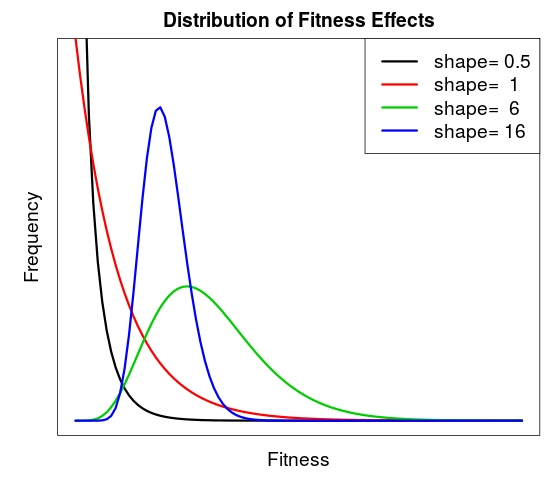
\includegraphics[width=7cm]{./Images/Gamma_dist.jpeg}
  \centering
  \caption{Example of different Distribution of Fitness Effects (DFE) represented by a gamma distribution.
  Many distributions can be represented by modifying the shape parameter of a gamma distribution, from
  a leptokurtic (shape parameter less than 1) to an exponential (shape parameter equal to 1) or a
  skewed normal distribution (shape  greater than 1).
   }
  \label{fig:Gamma}
\end{figure}


The divergence at the neutral sites is then proportional to the mutation rate per site and the predicted divergence at the selected sites, in the absence of advantageous mutations, 
is proportional to the product of the mutation rate and the average fixation probability of a selected mutation, 
which is inferred based on the DFE and other parameters estimated from the polymorphism data analysis
	\citep{Eyre-Walker2009}.
The difference between the observed and predicted divergences therefore estimates the divergence due to adaptive substitutions.

Using this method Eyre-Walker and collaborators estimated that approximately 50\% of amino acid substitutions and approximately 20\% of substitutions in introns are adaptive
	\citep{Eyre-Walker2009}.

Messer and Petrov performed molecular evolution simulations to test if the estimates of different tests, like the MKT and the more sophisticated DFE-alpha, are accurate under different realistic gene-structure and selection scenarios
	\citep{Messer2013}.
More specifically, the authors wanted to test how accurate these methods are in presence of genetic draft (stochastic effects generated by recurrent selective sweeps at closely linked sites)
and background selection (interference among linked sites by lightly deleterious polymorphisms).

They found that in the presence of slightly deleterious mutations, MKT estimates of $\alpha$ are severely underestimated.
They also found that the DFE-alpha is very accurate to calculate alpha when changes is demography are considered \citep{Messer2013}, with the caveat that DFE can highly overestimate the demography changes when genetic draft (stochastic effects generated by recurrent selective sweeps at closely linked sites) or background selection (interference among linked sites caused by lightly deleterious polymorphisms) are present \citep{Messer2013}.

This is because genetic draft leaves similar signatures to a recent population expansion, namely distortions of the SFS at synomymous sites, and the DFE-alpha interprets these SFS distortions as being a consequence of demography and attempts to correct for it.
Importantly, this caveat in using the DFE-alpha is only relevant when demography changes wants to be estimated, but not when alpha is the parameter of interest, as in here.
